\documentclass[12pt]{article}
\raggedbottom

\usepackage[utf8]{inputenc}
\usepackage{graphicx}
\usepackage[italian]{babel}
\usepackage{csquotes}
\usepackage{lipsum}
\usepackage{fancyhdr}
\usepackage{pdfpages}
\usepackage{wrapfig}
\usepackage{float}
\usepackage{enumitem}
\usepackage{subcaption}
\usepackage{framed}
\usepackage{listings,xcolor}
\usepackage{inconsolata}
\usepackage{setspace}
\usepackage[T1]{fontenc}
\usepackage[hidelinks]{hyperref}
\usepackage{booktabs}
\usepackage{amsmath}
\usepackage[a4paper,width=160mm,top=25mm,bottom=25mm]{geometry}

\definecolor{shadecolor}{gray}{0.8}

\title{\textbf{\textsc{Progetto 1 bis}}\\Metodi del Calcolo Scientifico}

\author{Elisa Pioldi\\
        Mat. 856591}
\date{Giugno 2023}

\begin{document}

\maketitle

\section{Introduzione}

L'obiettivo del progetto qui presentato è l'implementazione di una libreria che esegua i solutori iterativi di \textbf{Jacobi}, \textbf{Gauss-Seidel}, \textbf{gradiente} e \textbf{gradiente coniugato}, che fornisca anche una serie di \textit{utility} per aiutare la raccolta di statistiche, la creazione di grafici, la stampa a schermo e il riutilizzo di codice.

La libreria è consultabile al repository \href{https://github.com/epi-xel/linear-solver}{\texttt{epi-xel/linear-solver}} su GitHub.

\section{Tecnologie utilizzate}

Si è scelto di utilizzare \textbf{Python} come linguaggio di programmazione con uno scopo ben specifico. Infatti, data la flessibilità che offre nell'implementazione software e l'ampia scelta di librerie per i grafici e il calcolo scientifico, era uno dei pochi linguaggi che permettesse uno sviluppo agile a 360 gradi con delle ottime librerie per la produzione di grafici.

Le principali librerie di Python che sono state quindi utilizzate per l'implementazione vengono descritte di seguito:
\begin{itemize}
    \item \textbf{Scipy} e \textbf{Cholmod}, per la gestione delle \textit{matrici sparse}: il package \texttt{scipy.sparse} offre infatti un'ampia gamma di funzioni per trattare le matrici sparse, dalla lettura di file formato \texttt{.mtx}, all'esecuzione di operazioni base tra matrici; \texttt{sksparse.cholmod} permette invece di utilizzare il metodo di Choleski su matrici sparse.
    \item \textbf{Pandas}, \textbf{Matplotlib} e \textbf{Seaborn}, per l'analisi dei risultati, produzione di tabelle riassuntive e grafici.
\end{itemize}

\section{Struttura della libreria}

Il progetto si compone di due parti: una libreria e un eseguibile con un'interfaccia da linea di comando.

\subsection{Libreria \texttt{linearsolver}}

Data la complessità dell'idea progettuale, si è voluta strutturare la libreria in tre distinti moduli principali, ciascuno di essi contenente sottomoduli più specifici:

\begin{enumerate}
    \item \textbf{Helpers}: modulo dedicato alla definizione di classi di oggetti utilizzati per supportare/aiutare l'esecuzione di altri metodi 
    \item \textbf{Methods}: modulo che implementa gli algoritmi veri e propri per la risoluzione dei sistemi lineari
    \item \textbf{Utils}: modulo adibito all'implementazione di funzioni di varia natura, come per la stampa a schermo dei risultati e l'analisi di questi ultimi
\end{enumerate}

Si è cercato inoltre di coniugare la flessibilità di Python per il calcolo numerico con il suo paradigma procedurale e l'implementazione di classi focalizzate al disaccoppiamento delle funzioni della libreria che seguissero i più classici design patterns, con la programmazione ad oggetti. L'obiettivo era di mantenere la semplicità caratteristica di Python nelle funzioni base della libreria e arricchendo organicamente il resto delle funzioni ausiliarie per creare codice mantenibile, documentabile, facilmente utilizzabile ed incline a più livelli di astrazione.

\subsubsection{Helpers} \label{sec:helpers}

Tra i sottomoduli qui presenti, le classi di oggetti più interessanti che vengono definite sono: 
\begin{itemize}
    \item \texttt{LinearSystemHelper}: classe di oggetti che permette la memorizzazione di alcune variabili utili durante l'esecuzione dei metodi per la risoluzione dei sistemi, come la matrice $A$, il vettore $b$, il vettore soluzione $x$, il vettore soluzione esatta $x_{true}$ ed eventuali variabili specifiche per il metodo chiamato.
    \item \texttt{LinearSystemResult}: classe di oggetti per l'incapsulamento dei risultati ottenuti dagli algoritmi di risoluzione; in particolar modo viene salvato il vettore soluzione, il tempo di esecuzione, il numero di iterazioni e l'errore relativo.
    \item \texttt{ResultsStats}: classe di oggetti che si comporta similmente ad un \textit{dataframe} per la memorizzazione delle statistiche sui risultati, contenente alcuni metodi che permettono l'aggiunta di ulteriori statistiche o operare la fusione con un altro oggetto della stessa classe. Segue il design pattern \textit{builder}, dal momento che cerca di ottimizzare la costruzione iterativa del dataframe, che sarebbe altrimenti molto onerosa e si comporta anche da \textit{mediator} tra i moduli per la produzione e l'elaborazione dei risultati.
\end{itemize}

\subsubsection{Methods} \label{sec:methods}

Volendo applicare il design pattern \textit{strategy}, questo modulo contiene tre sottomoduli principali:
\begin{itemize}
    \item \texttt{base\_solver}: data la struttura comune di ciascun metodo si sono raccolte in questo modulo le funzioni condivise dai metodi.
    \item \texttt{update}: in questo modulo sono raccolte le funzioni di update distinte per ciascun metodo.
    \item \texttt{methods\_collector}: il modulo funge, in termini di design patterns, da \textit{facade}, raccogliendo una serie di funzioni ausiliarie che permettono l'esecuzione di tutti i metodi per un singolo input con una certa tolleranza e, utilizzando \texttt{print\_utils} (cfr. sezione \ref{sec:utils}) stampa a schermo i risultati.
\end{itemize}

Si approfondiscono di seguito i primi due moduli dedicati al cuore vero e proprio del progetto.

\paragraph{\texttt{base\_solver}} Il modulo si avvale di una funzione principale che contiene la struttura base degli algoritmi iterativi: la funzione prende in ingresso  $A$, $b$, $x$, la tolleranza, il massimo numero di iterazioni e l'elemento di un'enumerazione (sempre definita in questo stesso modulo), che definisce il metodo che si desidera eseguire. Il metodo al suo interno prima di tutto si avvale di un metodo ausiliario che converte il valore dell'enumerazione nella corrispondente funzione di update (definita nel modulo omonimo), poi, seguendo l'implementazione classica degli algoritmi iterativi, calcola il risultato, il tempo di esecuzione e il numero di iterazioni, servendosi durante le iterazioni dell'oggetto della classe \texttt{LinearSystemHelper} e incapsulando alla fine il risultato in un oggetto della classe \texttt{LinearSystemResult}, che restituisce al chiamante. Il vettore soluzione è inizializzato all'inizio del metodo come un vettore di tutti 0.

All'interno del modulo sono anche definite due funzioni ausiliare, di cui una calcola ad ogni iterazione la convergenza dell'algoritmo, secondo la seguente formula:

\[
    \frac{\Vert Ax^{(k)}-b \Vert}{\Vert b \Vert} < \texttt{tol}
\]

L'altra funzione invece viene eseguita prima di tutto per stabilire se la matrice è simmetrica e definita positiva, attraverso l'esecuzione del metodo di Choleski messo a disposizione dalla libreria \texttt{cholmod}: eventuali eccezioni vengono catturate e il controllo viene restituito al chiamante, stampando a schermo un messaggio di errore.

\paragraph{\texttt{update}} Questo modulo definisce le operazioni di update per ciascun metodo: \textbf{Jacobi}, \textbf{Gauss-Seidel}, \textbf{gradiente} e \textbf{gradiente coniugato}. Ciascuna delle funzioni principali accetta in ingresso un oggetto della classe \texttt{LinearSystemHelper}, su cui effettuano le operazioni di modifica e aggiornamento. 

Per ciascun metodo sono state utilizzate le operazioni base tra matrici sparse offerte dal package \texttt{scipy.sparse}. 

Ovviamente non è mai stata utilizzata la funzione per calcolare la matrice inversa, parte integrante di Gauss-Seidel e Jacobi: relativamente a Gauss-Seidel si è implementata a parte nella libreria una funzione che eseguisse la sostituzione in avanti (metodo \texttt{forward\_substitution}) dopo aver calcolato la matrice triangolare inferiore di A; Jacobi invece vede il calcolo della matrice inversa come la matrice diagonale con i coefficienti che sono i reciproci di quelli di P, matrice diagonale ricavata da A.

Per i metodi iterativi non stazionari l'unica nota implementativa va riferita al gradiente coniugato: questo update richiede infatti in input, oltre al vettore x, altre due variabili (che si sono chiamate \texttt{r} e \texttt{p}): l'oggetto \texttt{LinearSystemHelper} nel caso del gradiente coniugato vede pertanto l'aggiunta ai suoi attributi di queste variabili.

\subsubsection{Utils} \label{sec:utils}

I moduli di \textit{utility} sono:
\begin{itemize}
    \item \texttt{analize}: modulo che implementa la realizzazione di grafici ed esportazione di tabelle sulla base dei risultati ottenuti dagli algoritmi che implementano i metodi. Per interfacciarsi al metodo principale di questo modulo, \texttt{export\_results()}, è necessario utilizzare un oggetto della classe \texttt{ResultsStats} che incapsula i dati dei risultati e facilita la loro gestione tra le varie funzioni.
    \item \texttt{print\_utils}: modulo che raccoglie una serie di funzioni che permettono la stampa a schermo dei risultati ottenuti dai metodi. Per interfacciarsi al metodo principale di questo modulo si deve impiegare un oggetto della classe \texttt{LinearSystemResult}.
    \item \texttt{constants}: modulo dove sono contenute alcune costanti utilizzate nell'intero programma.
\end{itemize}

\subsection{Eseguibile}

Una volta implementata la libreria, si è voluto produrre un eseguibile che avesse un'interfaccia intuitiva da linea di comando. Eseguendo il file con il comando \texttt{-{}-help} (oppure se non si inserisce nulla) si ottiene l'output rappresentato nella figura \ref{fig:cli-1}.

\begin{figure}[H]
    \begin{center}
    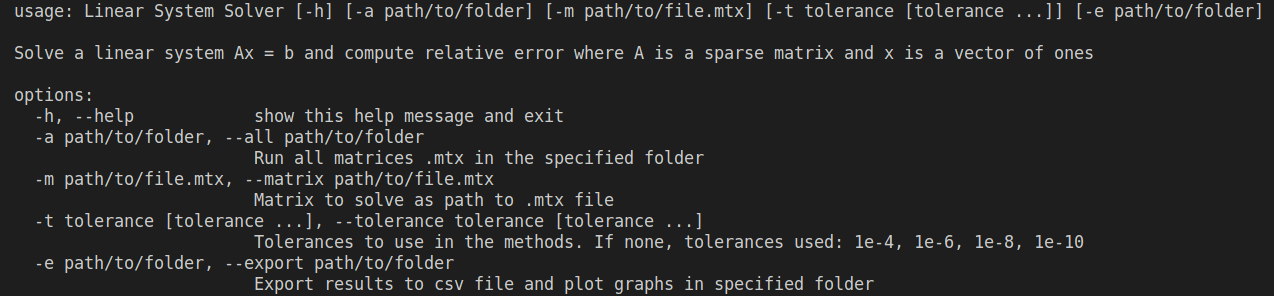
\includegraphics[width=\textwidth]{images/program-cli.png}
    \caption{Interfaccia da linea di comando del programma.}
    \label{fig:cli-1}
    \end{center}
\end{figure}

Da linea di comando è pertanto possibile inserire una o più matrici con diverse tolleranze e ottenere un output sia sul terminale, sia su file, con alcuni grafici e file CSV che riassumono l'esecuzione dei metodi.

\begin{shaded}
Per semplicità da linea di comando è possibile dare in input solo matrici, dato che all'interno dell'eseguibile viene calcolato $Ax = b$ dove $x$ è un vettore di soli uno. All'interno del file è però possibile sovrascrivere il vettore $x$ o $b$ con qualsiasi vettore desiderato.
\end{shaded}

Per ciascun sistema lineare in input viene calcolata la soluzione con ciascuna tolleranza e ciascun metodo, avvalendosi del modulo \texttt{methods\_collector} descritto nella sezione \ref{sec:methods}. Durante l'esecuzione degli algoritmi vengono stampati a schermo di volta in volta i risultati, come esemplificato dalla figura \ref{fig:cli-2}.

\begin{figure}[H]
    \begin{center}
    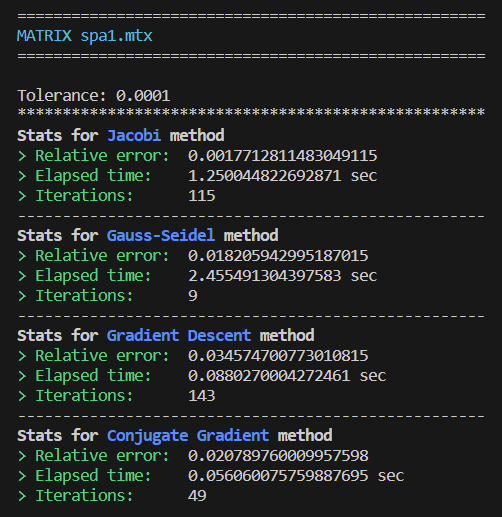
\includegraphics[scale=0.8]{images/output-cli.png}
    \caption{Output su terminale dopo l'esecuzione di \texttt{spa1.mtx} con tolleranza 0.0001.}
    \label{fig:cli-2}
    \end{center}
\end{figure}

%%%%% ANALISI RISULTATI %%%%%

\section{Analisi dei risultati}

Il programma sopra descritto ha ricevuto quindi come input le matrici di test \texttt{spa1.mtx}, \texttt{spa2.mtx}, \texttt{vem1.mtx} e \texttt{vem2.mtx}.
Per analizzare i risultati dell'implementazione dei metodi è stato necessario prima di tutto ottenere una panoramica delle proprietà di ciascuna matrice, come si può osservare nella tabella \ref{table:mat-stats}.

\begin{table}[!ht]
    \centering
    \begin{tabular}{ccc}
    \toprule
        \textbf{Matrix} & \textbf{Size} & \textbf{Density} \\ 
        \midrule
        spa1.mtx & 1000 & 0.182264 \\ 
        spa2.mtx & 3000 & 0.181304 \\ 
        vem1.mtx & 1681 & 0.004736 \\ 
        vem2.mtx & 2601 & 0.003137 \\ 
    \bottomrule
    \end{tabular}
    \caption{Dimensioni e densità delle matrici coinvolte.}
    \label{table:mat-stats}
\end{table}

L'esecuzione degli algoritmi implementati ha poi prodotto i risultati rappresentati nelle tabelle \ref{table:spa1-stats}, \ref{table:spa2-stats}, \ref{table:vem1-stats} e \ref{table:vem2-stats} divise per matrici.

Per un confronto più immediato si osservino i grafici a barre in figura \ref{fig:tie-b}, dove vengono messi a confronto i metodi con il numero di iterazioni, il tempo impiegato e l'errore relativo, divisi per tolleranza. 
Si noti che in tutti i grafici a barre qui presentati la scala dell'asse y è logaritmica.

\begin{figure}[!ht]
    \begin{center}
    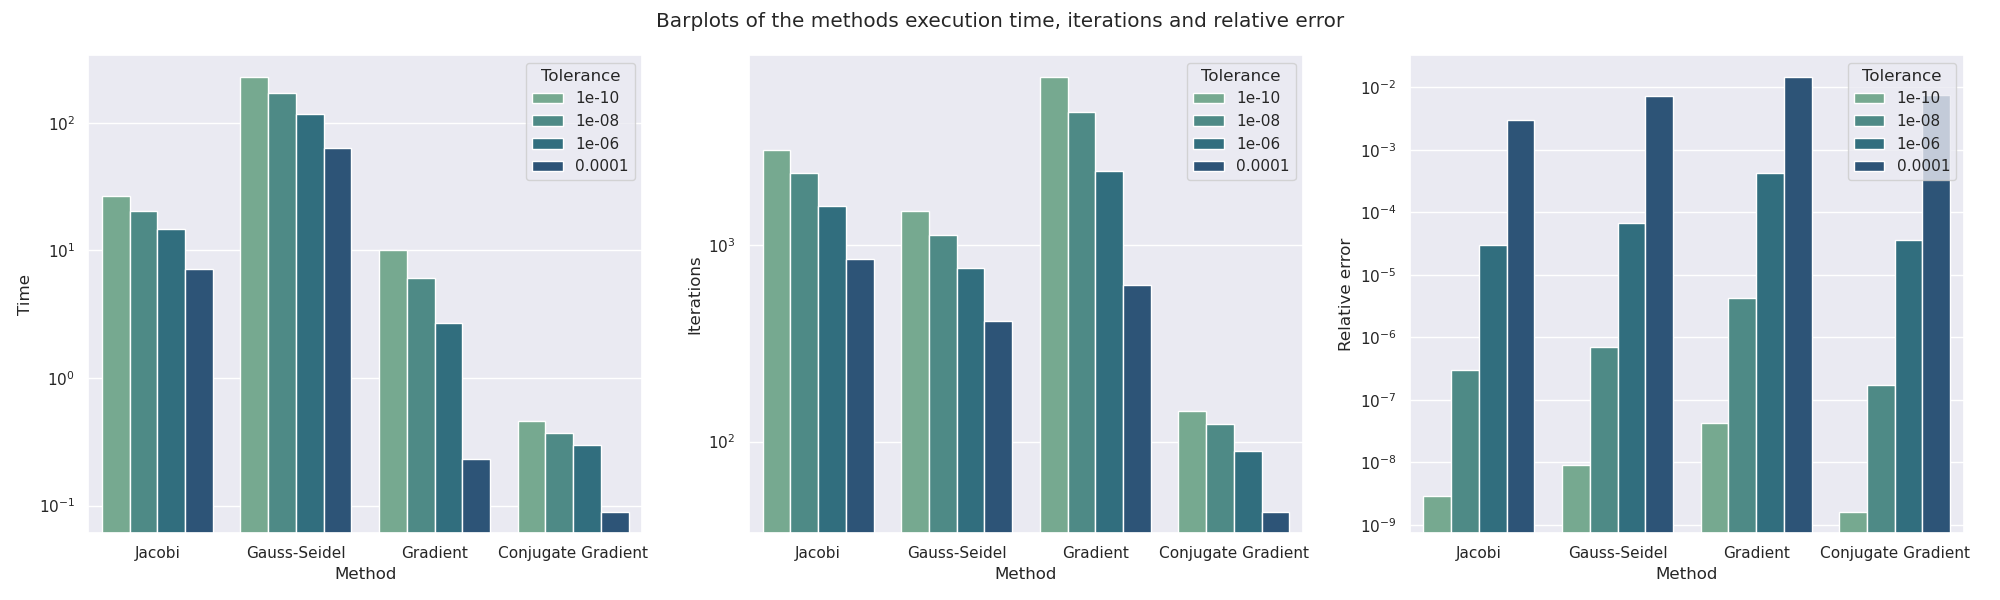
\includegraphics[width=\textwidth]{images/time-iterations-error_barplots.png}
    \caption{Grafici a barre del tempo di esecuzione, iterazioni ed errore relativo di ciascun metodo.}
    \label{fig:tie-b}
    \end{center}
\end{figure}

Banalmente si può vedere che diminuendo la tolleranza cresce esponenzialmente il tempo di esecuzione, il numero di iterazioni e diminuisce esponenzialmente l'errore relativo. In particolar modo l'errore relativo più basso che osserviamo è con il metodo del gradiente coniugato, che si distanzia in alcuni casi dagli altri anche di un paio di ordini di grandezza, seguito subito dal metodo di Jacobi.
Più interessante è il confronto tra i vari metodi e il tempo: Gauss-Seidel sembra essere il metodo che impiega più tempo, mentre il gradiente coniugato è il più veloce. Una possibile spiegazione della lentezza di Gauss-Seidel è l'utilizzo dell'algoritmo della sostituzione in avanti non ottimizzata per matrici sparse, che può aumentare significativamente il tempo di esecuzione.
Relativamente al numero di iterazioni è però il gradiente il metodo che vede più iterazioni, di contro il gradiente coniugato converge con un minimo numero di iterazioni. Gauss-Seidel per numero di iterazioni è molto buono, appena dietro al metodo del gradiente coniugato, a maggior riprova che l'utilizzo della sostituzione in avanti non della libreria di Python lo penalizza.

Nonostante questa prima analisi dà già un'idea delle performance degli algoritmi, osservando i dati nelle tabelle si può intuire una correlazione tra la dimensione e la densità della matrice con il tempo e il numero di iterazioni a seconda dei vari metodi impiegati. 
Confermiamo questi sospetti osservando le matrici di correlazione in figura \ref{fig:cormat}.

\begin{figure}[!ht]
    \begin{center}
    \hspace*{-2cm}   
    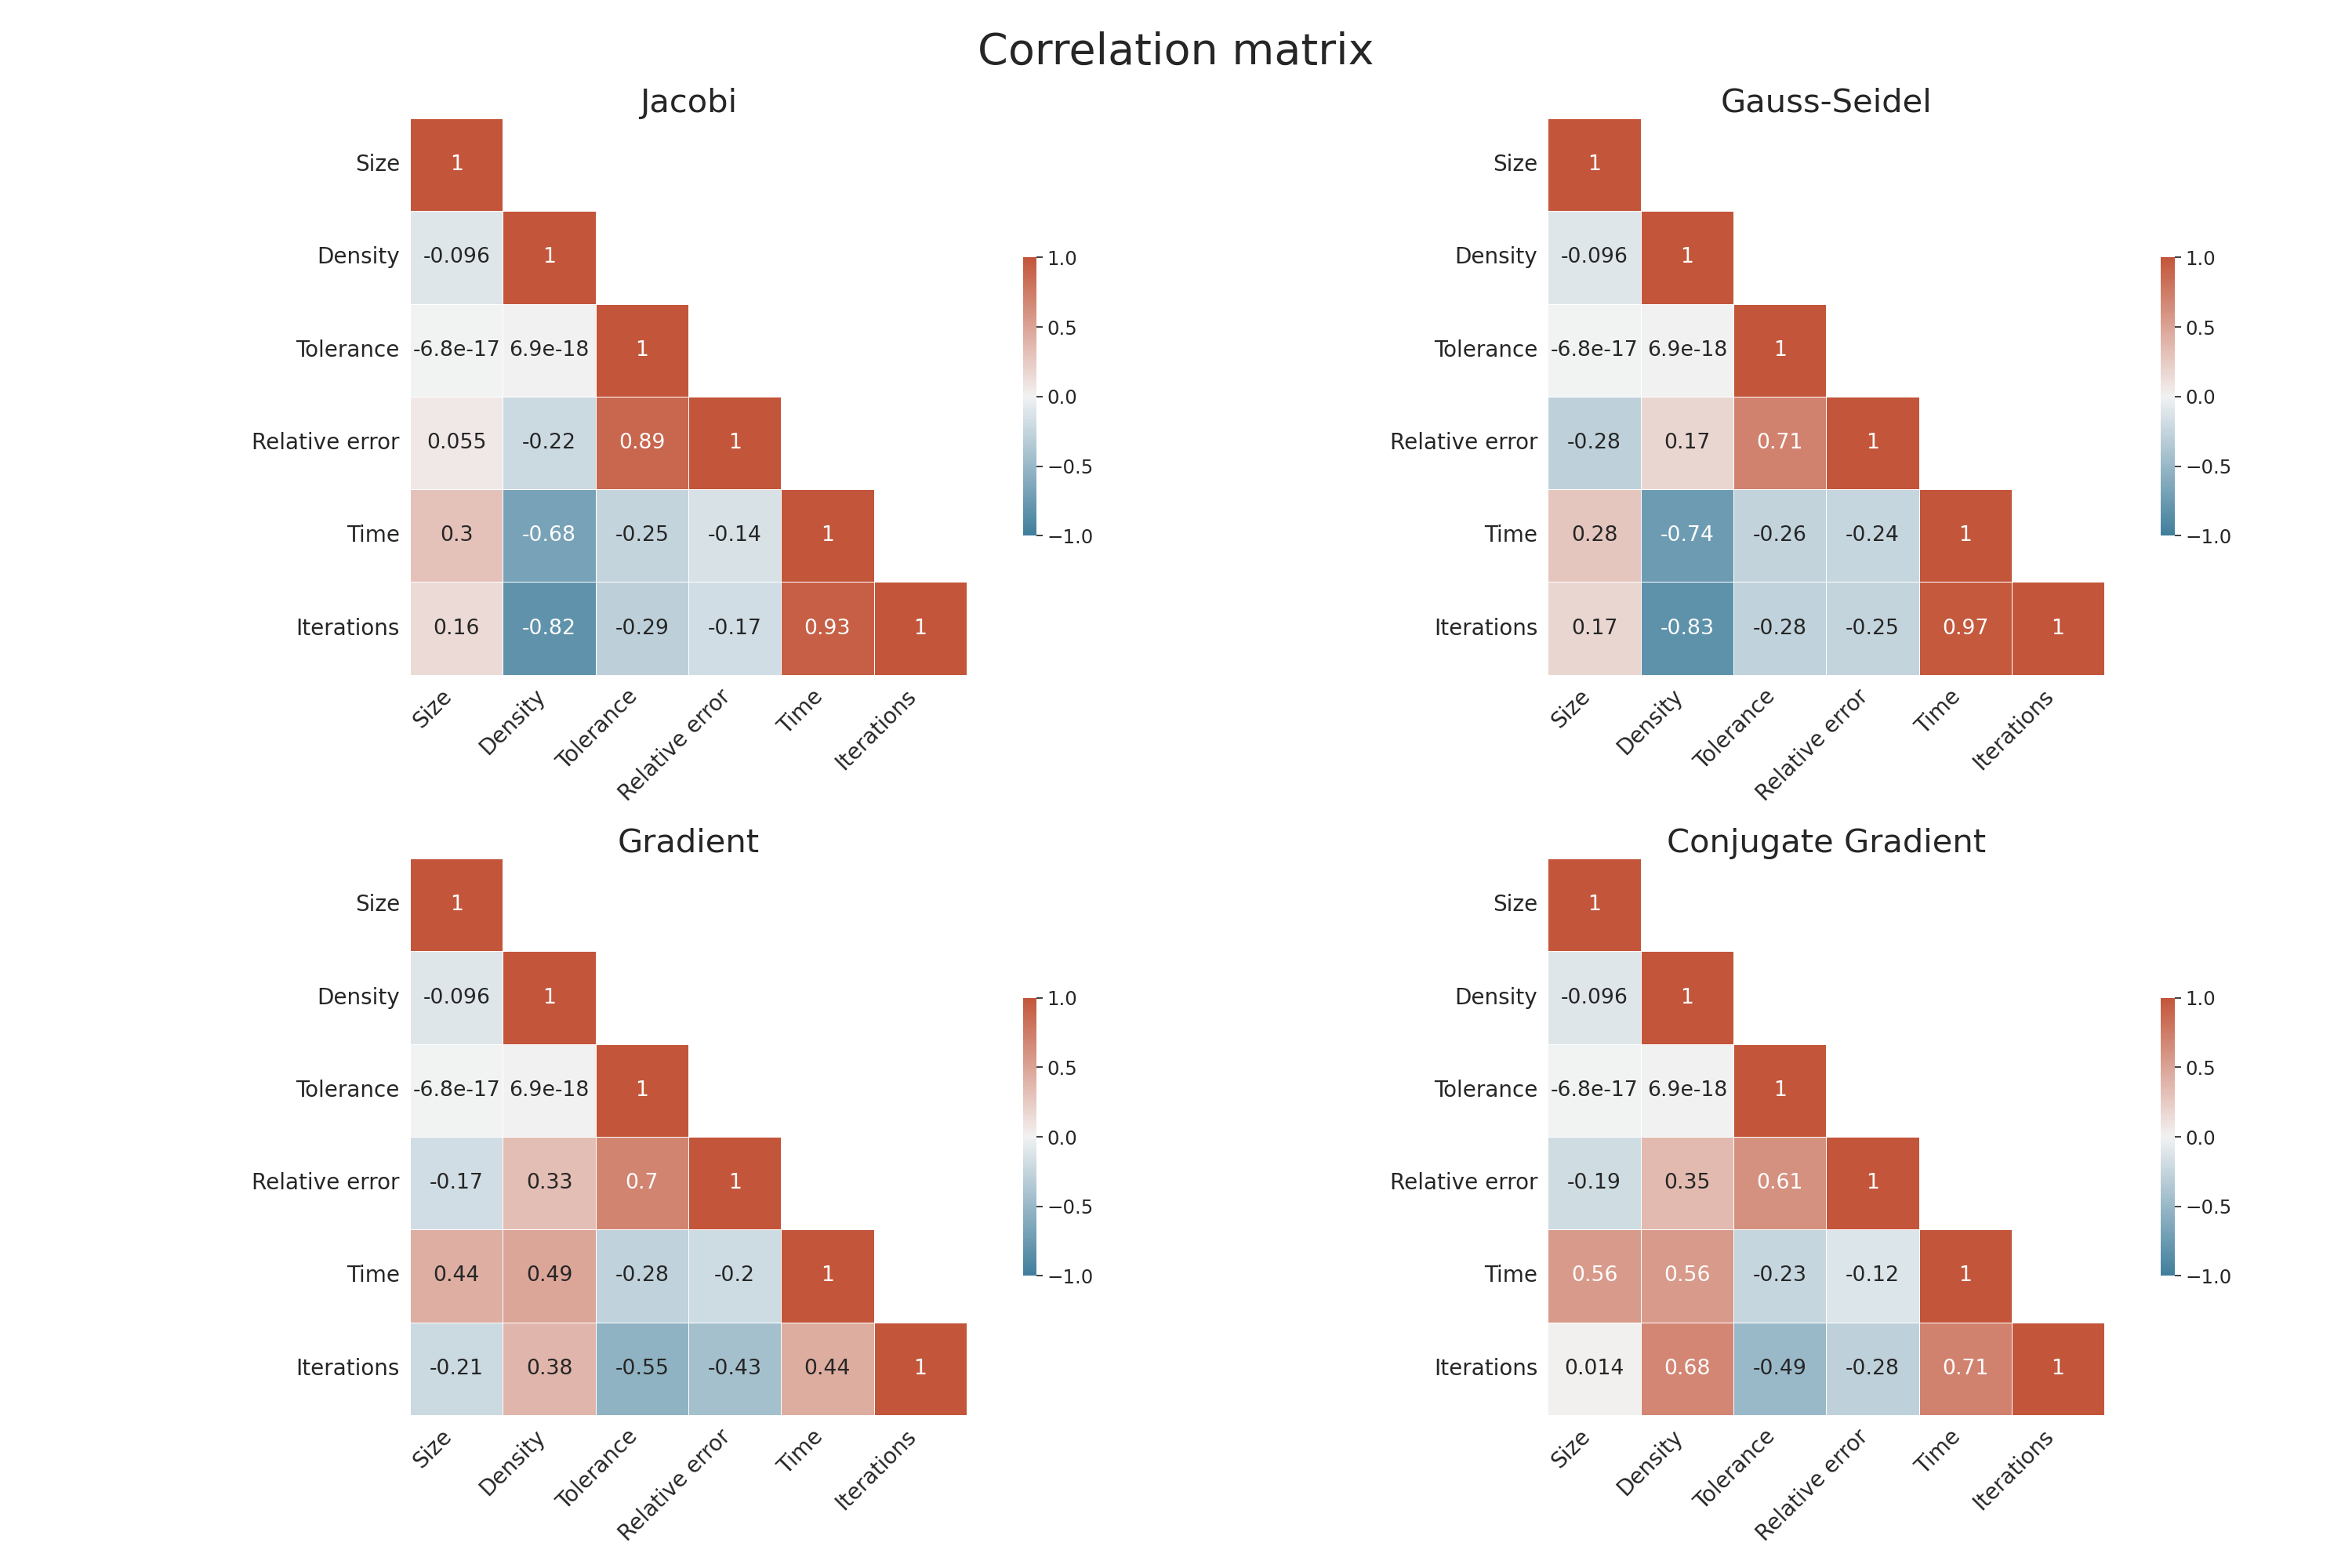
\includegraphics[scale=0.25]{images/heatmaps.png}
    \caption{Matrici di correlazione dei risultati di ciascun metodo.}
    \label{fig:cormat}
    \end{center}
\end{figure}

\paragraph{Jacobi}
Il metodo di Jacobi vede una forte correlazione negativa tra densità e iterazioni e una modesta correlazione sempre negativa tra densità e tempo. La dimensione risulta invece pressoché ininfluente. Jacobi è quindi più adatto a matrici più dense di grandi dimensioni.

\paragraph{Gauss-Seidel}
Gauss-Seidel si comporta similmente a Jacobi con una forte correlazione negativa tra densità e iterazioni e tra densità e tempo. Anche Gauss-Seidel sembra essere più adatto a matrici dense molto grandi.

\paragraph{Gradiente}
Il metodo del gradiente invece trova una modesta correlazione positiva tra densità e iterazioni e tra densità e tempo. La dimensione è invece influente sul tempo con una correlazione positiva. Questo metodo è quindi destinato alla risoluzione di matrici poco dense ma non di grandi dimensioni.

\paragraph{Gradiente coniugato}
Il gradiente coniugato accentua la tendenza del gradiente con una correlazione positiva tra densità e iterazioni, tra densità e tempo e tra dimensione e tempo.
Anche il gradiente coniugato è pertanto più adatto a matrici poco dense e non di grandi dimensioni.

Le osservazioni fatte qui sopra vengono mostrate intuitivamente dai grafici a barre nelle figure \ref{fig:di-b} e \ref{fig:dt-b}.

\begin{figure}[!ht]
    \begin{center}
    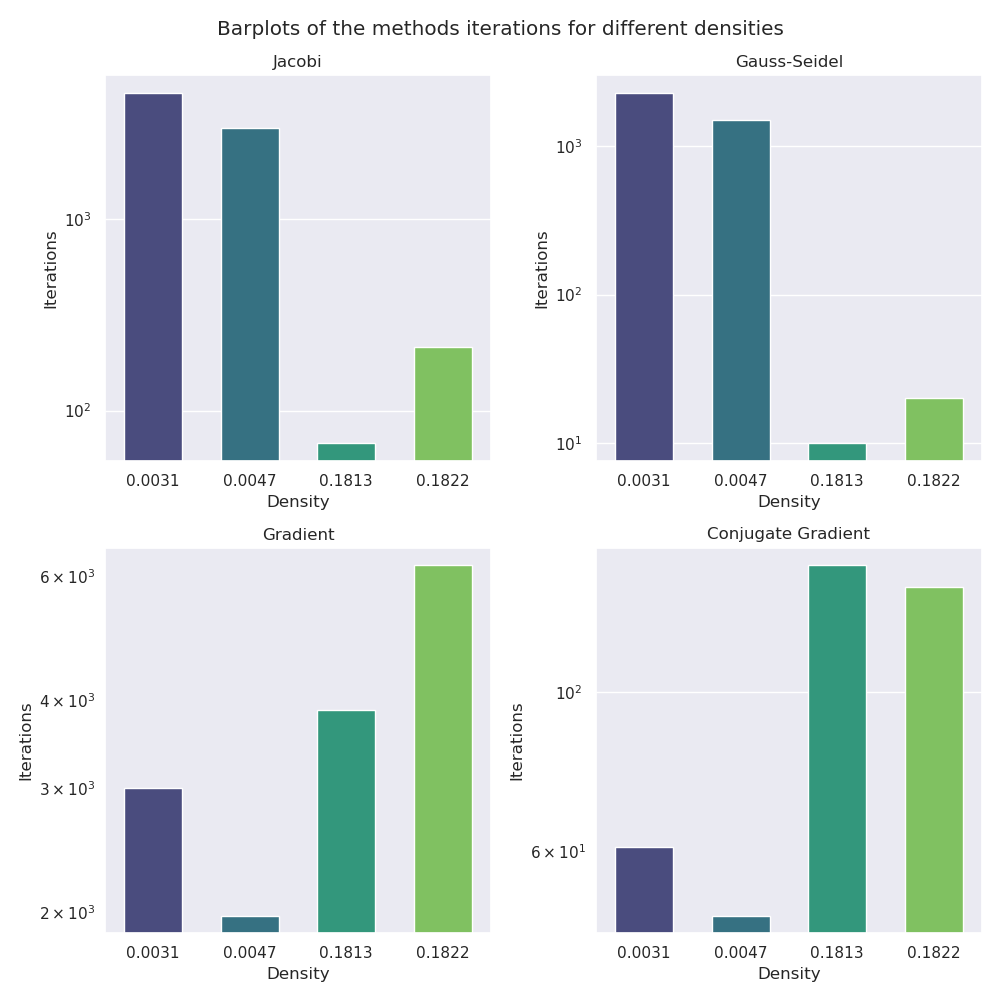
\includegraphics[scale=0.6]{images/density-iterations_barplots.png}
    \caption{Grafici a barre del confronto tra densità e iterazioni per ciascun metodo.}
    \label{fig:di-b}
    \end{center}
\end{figure}

\begin{figure}[!ht]
    \begin{center}
    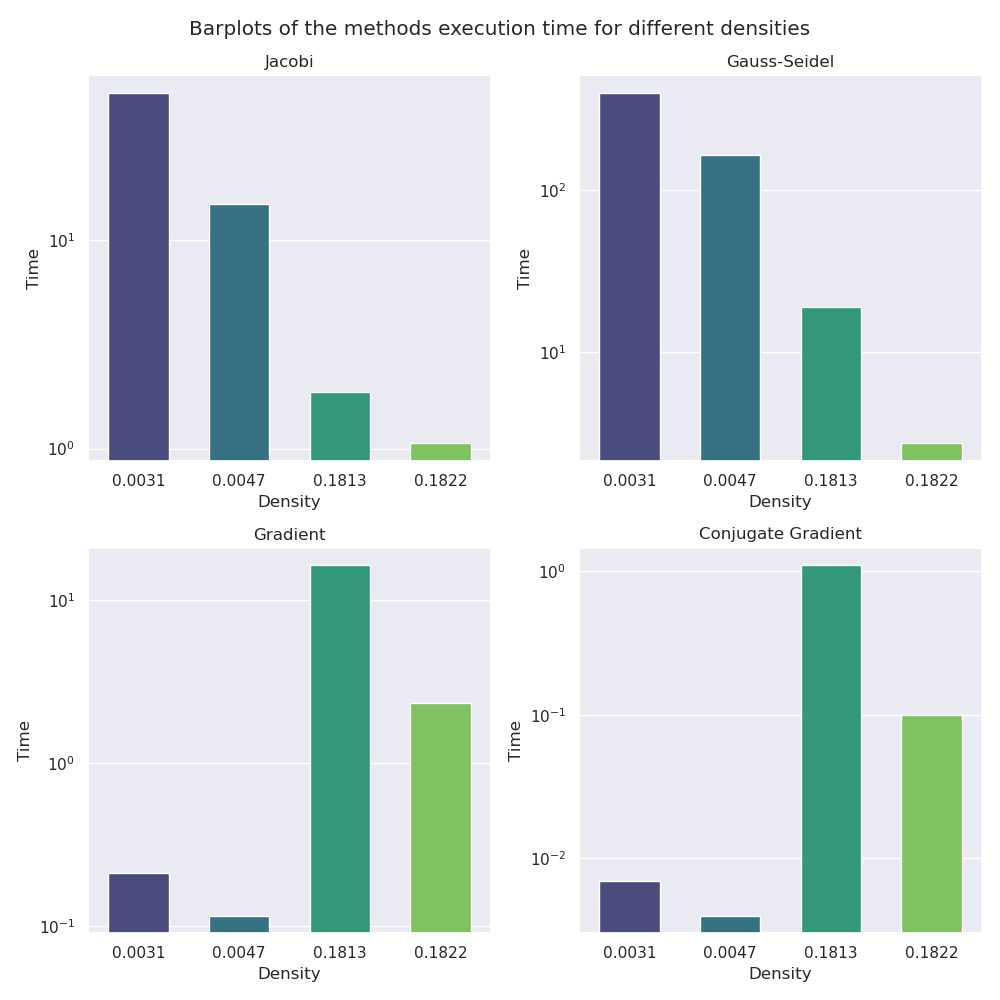
\includegraphics[scale=0.6]{images/density-time_barplots.png}
    \caption{Grafici a barre del confronto tra densità e tempo per ciascun metodo.}
    \label{fig:dt-b}
    \end{center}
\end{figure}

\begin{table}[!ht]
    \centering
    \begin{tabular}{ccccc}
    \toprule
    \multicolumn{5}{c}{\texttt{spa1.mtx}}\\
    \midrule
        \textbf{Method} & \textbf{Tolerance} & \textbf{Time (sec)} & \textbf{Iterations} & \textbf{Relative error} \\ \midrule
        Jacobi & 0.0001 & 0.6279 & 115 & 0.0017 \\ 
        Gauss-Seidel & 0.0001 & 1.2264 & 9 & 0.0182 \\ 
        Gradient & 0.0001 & 0.0671 & 143 & 0.0345 \\ 
        Conjugate Gradient & 0.0001 & 0.0421 & 49 & 0.0207 \\ \midrule
        Jacobi & 1e-06 & 0.8952 & 181 & 1.7979-05 \\ 
        Gauss-Seidel & 1e-06 & 2.276 & 17 & 0.0001 \\ 
        Gradient & 1e-06 & 1.2214 & 3577 & 0.0009 \\ 
        Conjugate Gradient & 1e-06 & 0.0955 & 134 & 2.5529e-05 \\ \midrule
        Jacobi & 1e-08 & 1.1803 & 247 & 1.8249e-07 \\ 
        Gauss-Seidel & 1e-08 & 3.2228 & 24 & 1.7097e-06 \\ 
        Gradient & 1e-08 & 3.3928 & 8233 & 9.8163e-06 \\ 
        Conjugate Gradient & 1e-08 & 0.1219 & 177 & 1.3198e-07 \\ \midrule
        Jacobi & 1e-10 & 1.5406 & 313 & 1.8524e-09 \\ 
        Gauss-Seidel & 1e-10 & 4.1819 & 31 & 2.2480e-08 \\ 
        Gradient & 1e-10 & 4.7005 & 12919 & 9.8203e-08 \\ 
        Conjugate Gradient & 1e-10 & 0.1411 & 200 & 1.2077e-09 \\  \bottomrule
    \end{tabular}
    \caption{Risultati dell'esecuzione degli algoritmi su \texttt{spa1.mtx}}
    \label{table:spa1-stats}
\end{table}

\begin{table}[!ht]
    \centering
    \begin{tabular}{ccccc}
    \toprule
    \multicolumn{5}{c}{\texttt{spa2.mtx}}\\
    \midrule
        \textbf{Method} & \textbf{Tolerance} & \textbf{Time (sec)} & \textbf{Iterations} & \textbf{Relative error} \\ \midrule
        Jacobi & 0.0001 & 1.0455 & 36 & 0.0017 \\ 
        Gauss-Seidel & 0.0001 & 10.0109 & 5 & 0.0025 \\ 
        Gradient & 0.0001 & 0.696 & 161 & 0.0181 \\ 
        Conjugate Gradient & 0.0001 & 0.3088 & 42 & 0.0098 \\ \midrule
        Jacobi & 1e-06 & 1.5683 & 57 & 1.6667e-05 \\ 
        Gauss-Seidel & 1e-06 & 16.0884 & 8 & 5.1416e-05 \\ 
        Gradient & 1e-06 & 9.2137 & 1949 & 0.0006 \\ 
        Conjugate Gradient & 1e-06 & 1.0808 & 122 & 0.0001 \\ \midrule
        Jacobi & 1e-08 & 2.1628 & 78 & 1.5728e-07 \\ 
        Gauss-Seidel & 1e-08 & 21.7616 & 12 & 2.7943e-07 \\ 
        Gradient & 1e-08 & 20.5314 & 5087 & 6.8652e-06 \\ 
        Conjugate Gradient & 1e-08 & 1.3391 & 196 & 5.5866e-07 \\ \midrule
        Jacobi & 1e-10 & 2.6861 & 99 & 1.4842e-09 \\ 
        Gauss-Seidel & 1e-10 & 27.3729 & 15 & 5.5707e-09 \\ 
        Gradient & 1e-10 & 35.2379 & 8285 & 6.9378e-08 \\ 
        Conjugate Gradient & 1e-10 & 1.673 & 240 & 5.32423e-09 \\   \bottomrule
    \end{tabular}
    \caption{Risultati dell'esecuzione degli algoritmi su \texttt{spa2.mtx}}
    \label{table:spa2-stats}
\end{table}

\begin{table}[!ht]
    \centering
    \begin{tabular}{ccccc}
    \toprule
    \multicolumn{5}{c}{\texttt{vem1.mtx}}\\
    \midrule
        \textbf{Method} & \textbf{Tolerance} & \textbf{Time (sec)} & \textbf{Iterations} & \textbf{Relative error} \\ \midrule
        Jacobi & 0.0001 & 5.878 & 1314 & 0.0035 \\ 
        Gauss-Seidel & 0.0001 & 74.7871 & 659 & 0.0035 \\ 
        Gradient & 0.0001 & 0.0613 & 890 & 0.0027 \\ 
        Conjugate Gradient & 0.0001 & 0.0031 & 38 & 4.0827e-05 \\ \midrule
        Jacobi & 1e-06 & 15.5031 & 2433 & 3.5400e-05 \\ 
        Gauss-Seidel & 1e-06 & 134.0643 & 1218 & 3.5266e-05 \\ 
        Gradient & 1e-06 & 0.0856 & 1612 & 2.7133e-05 \\ 
        Conjugate Gradient & 1e-06 & 0.0036 & 45 & 3.7323e-07 \\ \midrule
        Jacobi & 1e-08 & 16.8194 & 3552 & 3.5397e-07 \\ 
        Gauss-Seidel & 1e-08 & 194.8304 & 1778 & 3.5174e-07 \\ 
        Gradient & 1e-08 & 0.1472 & 2336 & 2.6953e-07 \\ 
        Conjugate Gradient & 1e-08 & 0.0044 & 53 & 2.8318e-09 \\ \midrule
        Jacobi & 1e-10 & 21.6583 & 4671 & 3.5394e-09 \\ 
        Gauss-Seidel & 1e-10 & 255.6368 & 2338 & 3.5082e-09 \\ 
        Gradient & 1e-10 & 0.1664 & 3058 & 2.7131e-09 \\ 
        Conjugate Gradient & 1e-10 & 0.0048 & 59 & 2.1917e-11 \\   \bottomrule
    \end{tabular}
    \caption{Risultati dell'esecuzione degli algoritmi su \texttt{vem1.mtx}}
    \label{table:vem1-stats}
\end{table}

\begin{table}[!ht]
    \centering
    \begin{tabular}{ccccc}
    \toprule
    \multicolumn{5}{c}{\texttt{vem2.mtx}}\\
    \midrule
        \textbf{Method} & \textbf{Tolerance} & \textbf{Time (sec)} & \textbf{Iterations} & \textbf{Relative error} \\ \midrule
        Jacobi & 0.0001 & 21.1842 & 1927 & 0.0049 \\ 
        Gauss-Seidel & 0.0001 & 166.5856 & 965 & 0.0049 \\ 
        Gradient & 0.0001 & 0.1007 & 1308 & 0.0038 \\ 
        Conjugate Gradient & 0.0001 & 0.005 & 47 & 5.7290e-05 \\ \midrule
        Jacobi & 1e-06 & 41.432 & 3676 & 4.9670e-05 \\ 
        Gauss-Seidel & 1e-06 & 320.5974 & 1840 & 4.9417e-05 \\ 
        Gradient & 1e-06 & 0.1817 & 2438 & 3.7914e-05 \\ 
        Conjugate Gradient & 1e-06 & 0.0069 & 56 & 4.7429e-07 \\ \midrule
        Jacobi & 1e-08 & 60.7174 & 5425 & 4.9656e-07 \\ 
        Gauss-Seidel & 1e-08 & 467.1627 & 2714 & 4.95832e-07 \\ 
        Gradient & 1e-08 & 0.2431 & 3566 & 3.8098e-07 \\ 
        Conjugate Gradient & 1e-08 & 0.0071 & 66 & 4.2999e-09 \\ \midrule
        Jacobi & 1e-10 & 80.6605 & 7174 & 4.9641e-09 \\ 
        Gauss-Seidel & 1e-10 & 633.3592 & 3589 & 4.9489e-09 \\ 
        Gradient & 1e-10 & 0.3212 & 4696 & 3.7987e-09 \\ 
        Conjugate Gradient & 1e-10 & 0.009 & 74 & 2.2476e-11 \\   \bottomrule
    \end{tabular}
    \caption{Risultati dell'esecuzione degli algoritmi su \texttt{vem2.mtx}}
    \label{table:vem2-stats}
\end{table}

\section{Conclusioni}

Gli obiettivi implementativi sono stati raggiunti: l'unica nota dolente la ritroviamo nei tempi di esecuzione di Gauss-Seidel con matrici poco dense, probabilmente a causa dell'implementazione della sostituzione in avanti nell'update del metodo.

L'interfaccia da linea di comando dell'eseguibile consente una buona facilità di utilizzo e la produzione di grafici risulta molto efficace per un'analisi post esecuzione.

In conclusione, i metodi implementati in questo progetto vedono preferire in generale come tempo computazionale e numero di iterazioni l'utilizzo del gradiente coniugato.

\end{document}
